\documentclass[11pt,a4paper]{article}

\usepackage{style2017}
\usepackage{hyperref}

\hypersetup{
    colorlinks =false,
    linkcolor=blue,
   linkbordercolor = 1 0 0
}
\newcounter{numexo}
\setcellgapes{1pt}

\begin{document}



\begin{NSI}
{Activité}{Les fonctions}
\end{NSI}

\section*{Introduction}
L'écriture d'un programme peut devenir très rapidement long avec des morceaux de codes qui se répètent. Pour rendre le programme plus lisible et éviter de réécrire des lignes de codes identiques, on peut dans de nombreux langages de programmation utiliser des \textbf{fonctions}.\medskip

Les fonctions regroupent en un même endroit les lignes de codes qui se répètent. Ensuite, les fonctions sont appelées quand le programme en a besoin.\medskip

Dans un exercice sur les boucles, nous avons été amenés à créer des dessins avec différents motifs qui pouvaient se répéter de nombreuses fois. On va réaliser les mêmes figures en utilisant des fonctions.

\subsubsection*{La syntaxe en python}


\begin{itemize}
\item Une fonction en python est introduite par le mot clef \textbf{def} suivi du nom de la fonction, de 2 parenthèses et les deux points :
\item Les instructions de la fonction sont toutes \textbf{indentées} à l'intérieur de la fonction
\item le résultat ou la valeur de la fonction est renvoyé au programme avec le mot clef \textbf{return}
\end{itemize}
\begin{center}
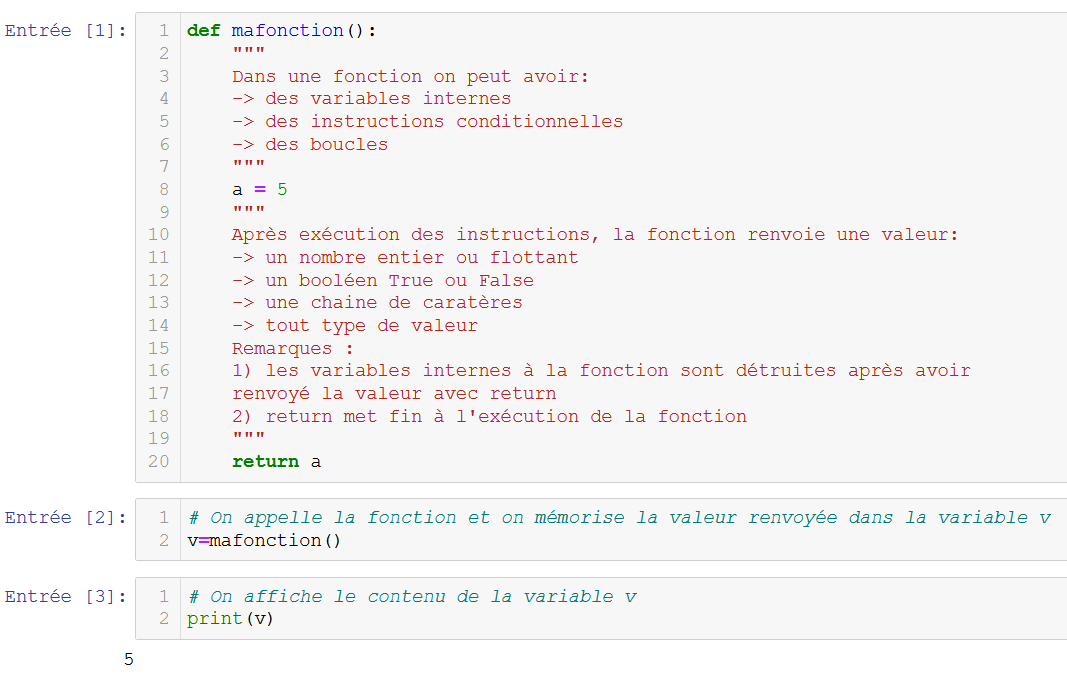
\includegraphics[scale=0.66]{img/mafonction.png}
\end{center}
Dans l'exemple ci-dessus:
\begin{itemize}
\item \textbf{Entrée [1]:} contient la fonction avec les instructions à réaliser lorsqu'elle est appelée;
\item \textbf{Entrée [2]:} on appelle la fonction et la valeur retournée sera affectée à la variable v;
\item \textbf{Entrée [3]:} on récupère la valeur de la variable v renvoyée par la fonction et on l'affiche.
\end{itemize}

\newpage
\section*{Partie 1 : avec une fonction}
Pour réaliser le dessin composé de 10 lignes de 10 fois la lettre X, on propose le programme suivant:

\begin{minipage}{14cm}
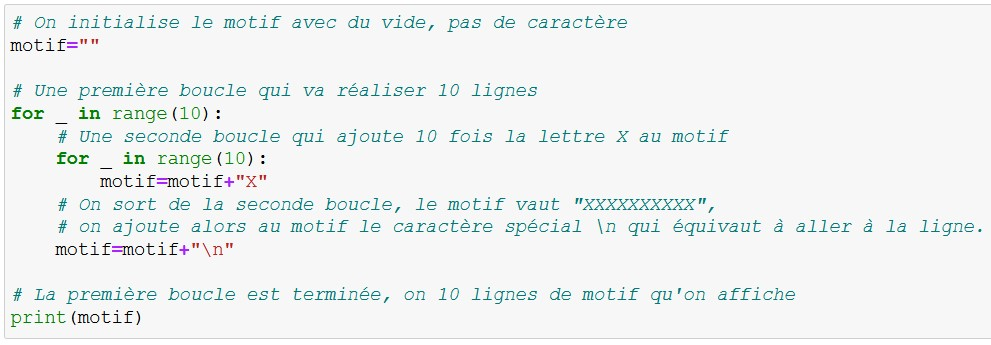
\includegraphics[scale=0.6]{img/bouclemotifX.jpg}
\end{minipage}\hfill
\begin{minipage}{2.6cm}
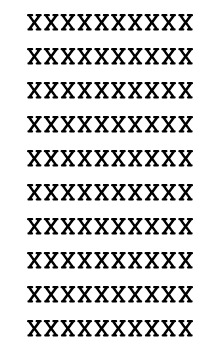
\includegraphics[scale=0.7]{img/carreX.jpg}
\end{minipage}\medskip

On va réaliser le même dessin en utilisant une fonction.

\begin{enumerate}
\item Créer la fonction \textbf{ligne\_X()} qui renvoie un motif composé de 10 fois la lettre \textbf{X} et du caractère spécial de retour à la ligne.
\item Écrire le programme ci-dessus en remplaçant la seconde boucle par l'appel à la fonction \textbf{ligne\_X()}. On utilisera une variable dessin à laquelle on affectera la valeur renvoyée par la fonction.
\item Vérifier que le dessin est bien réalisé.
\end{enumerate}

\section*{Partie 2 : une fonction et des paramètres}
La fonction précédente ne peut réaliser le dessin qu'avec 10 lignes de 10 \textbf{X}.\medskip

Il est possible de modifier cette valeur en passant un paramètre \textbf{n} à la fonction qui correspondra au nombre de X à afficher ainsi que le nombre de lignes du dessin.\medskip

\noindent Pour y parvenir, il faut:
\begin{enumerate}
\item Réécrire la fonction précédente en la renommant \textbf{ligne\_nX(n)}.
\begin{enumerate}
\item Ajouter le paramètre \textbf{n} entre les parenthèses de la fonction correspondant au nombre de X du motif.
\item Remplace la valeur 10 par le paramètre \textbf{n} dans la fonction.
\end{enumerate} 
\item Réécrire le programme en y insérant la fonction \textbf{ligne\_nX(n)} et en initialisant la valeur de n.
\item Vérifier votre programme en réalisant le dessin avec plusieurs valeurs de n.\medskip

\textbf{En supplément:}

\item On va modifier la fonction et le programme pour réaliser un dessin avec un autre caractère que le X.
\begin{enumerate}
\item  Ajouter un second paramètre \textbf{c} à votre fonction pour remplacer la lettre X par n'importe quel autre caractère.
\item Modifier le programme pour réaliser le dessin avec le caractère choisi.
\end{enumerate}
\item Ajouter des instructions pour que le nombre de lignes et le caractère soit saisi par l'utilisateur.
\end{enumerate}

\newpage
\section*{Partie 3 : un programme et plusieurs fonctions}

Pour réaliser la figure suivante, on peut utiliser plusieurs boucles et des print. 

Cette façon de faire n'est pas du tout optimisée.
\begin{center}
\begin{minipage}{8cm}
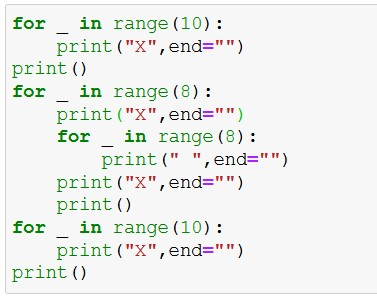
\includegraphics[scale=0.6]{img/bouclescarreXvide.jpg}
\end{minipage}
\begin{minipage}{4cm}
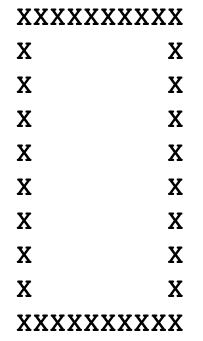
\includegraphics[scale=0.6]{img/carreX2.png}
\end{minipage}
\end{center}

Vous allez réécrire ce code en utilisant 2 fonctions:
\begin{itemize}
\item une fonction qui renvoie la première et la dernière ligne;
\item une fonction qui renvoie les lignes intermédiaires avec du vide;
\end{itemize}
Ci-dessous l'algorithme pour coder les deux fonctions et le programme:
\begin{center}
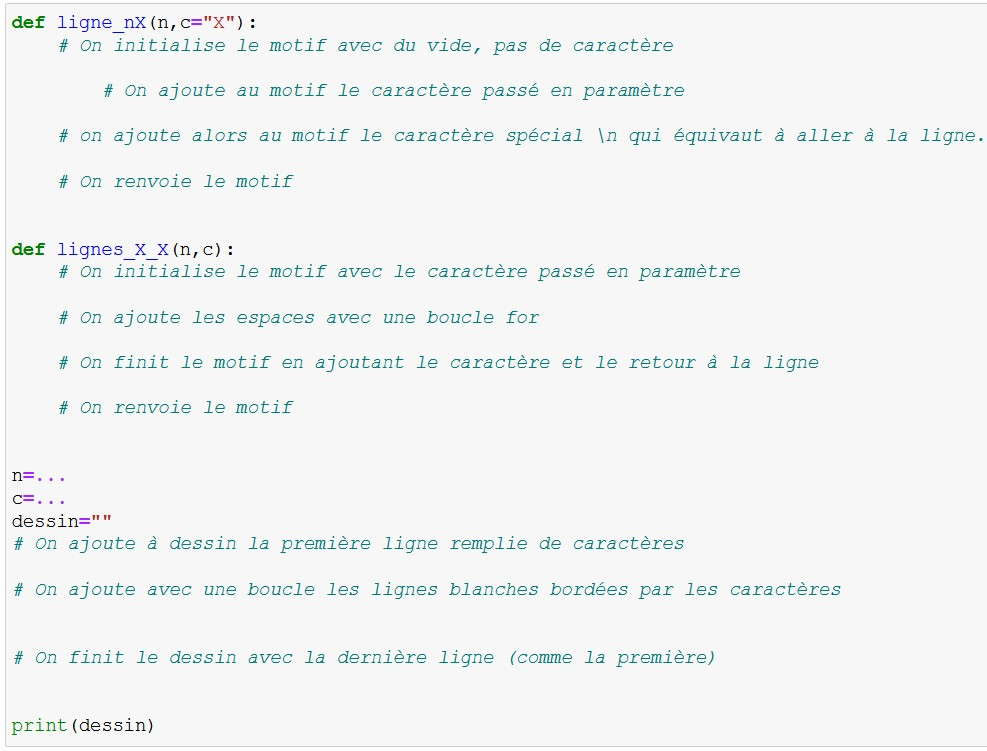
\includegraphics[scale=0.6]{img/algocarreXvide.jpg}
\end{center}
\begin{enumerate}
\item Écrire la première fonction en utilisant ce qui a déjà été fait;
\item Écrire la seconde fonction en suivant l'algorithme;
\item Terminer par le programme et faire des essais pour vérifier le bon fonctionnement.
\end{enumerate}

\newpage
\section*{Partie 4 : dernière figure}

On donne le programme et la figure suivante:

\begin{center}
\begin{minipage}{11cm}
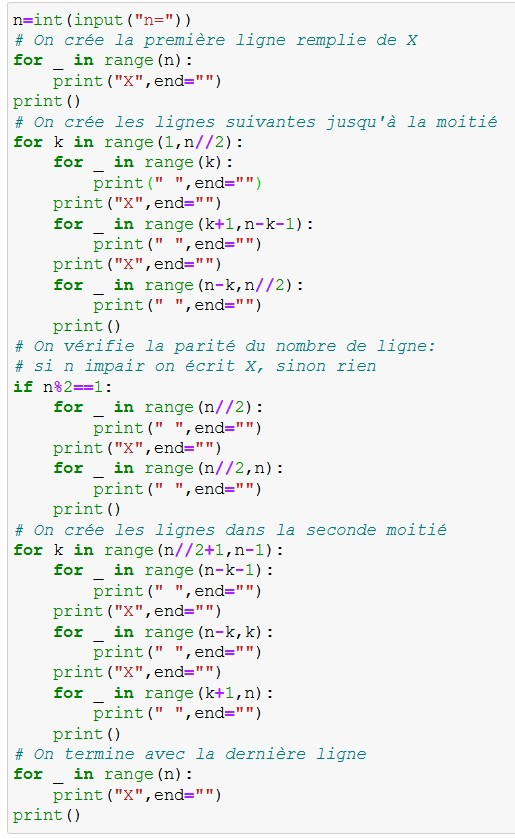
\includegraphics[scale=0.8]{img/bouclescarreXcroix.jpg}
\end{minipage}
\begin{minipage}{5cm}
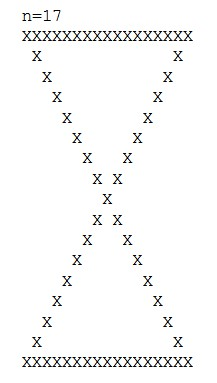
\includegraphics[scale=0.8]{img/carreXcroix.jpg}
\end{minipage}
\end{center}

Réécrire ce code en utilisant des fonctions.


\end{document}
